
%% bare_jrnl.tex
%% V1.4b
%% 2015/08/26
%% by Michael Shell
%% see http://www.michaelshell.org/
%% for current contact information.
%%
%% This is a skeleton file demonstrating the use of IEEEtran.cls
%% (requires IEEEtran.cls version 1.8b or later) with an IEEE
%% journal paper.
%%
%% Support sites:
%% http://www.michaelshell.org/tex/ieeetran/
%% http://www.ctan.org/pkg/ieeetran
%% and
%% http://www.ieee.org/

%%*************************************************************************
%% Legal Notice:
%% This code is offered as-is without any warranty either expressed or
%% implied; without even the implied warranty of MERCHANTABILITY or
%% FITNESS FOR A PARTICULAR PURPOSE! 
%% User assumes all risk.
%% In no event shall the IEEE or any contributor to this code be liable for
%% any damages or losses, including, but not limited to, incidental,
%% consequential, or any other damages, resulting from the use or misuse
%% of any information contained here.
%%
%% All comments are the opinions of their respective authors and are not
%% necessarily endorsed by the IEEE.
%%
%% This work is distributed under the LaTeX Project Public License (LPPL)
%% ( http://www.latex-project.org/ ) version 1.3, and may be freely used,
%% distributed and modified. A copy of the LPPL, version 1.3, is included
%% in the base LaTeX documentation of all distributions of LaTeX released
%% 2003/12/01 or later.
%% Retain all contribution notices and credits.
%% ** Modified files should be clearly indicated as such, including  **
%% ** renaming them and changing author support contact information. **
%%*************************************************************************


% *** Authors should verify (and, if needed, correct) their LaTeX system  ***
% *** with the testflow diagnostic prior to trusting their LaTeX platform ***
% *** with production work. The IEEE's font choices and paper sizes can   ***
% *** trigger bugs that do not appear when using other class files.       ***                          ***
% The testflow support page is at:
% http://www.michaelshell.org/tex/testflow/




\documentclass[journal]{IEEEtran}

%\usepackage{natbib} % Required to change bibliography style to APA
%
% If IEEEtran.cls has not been installed into the LaTeX system files,
% manually specify the path to it like:
% \documentclass[journal]{../sty/IEEEtran}


%-------------------------------------------
%New colors defined below
%\definecolor{codegreen}{rgb}{0,0.6,0}
%\definecolor{codegray}{rgb}{0.5,0.5,0.5}
%\definecolor{codepurple}{rgb}{0.58,0,0.82}
%\definecolor{backcolour}{rgb}{0.95,0.95,0.92}

%%Code listing style named "mystyle"
%\lstdefinestyle{mystyle}{
%	backgroundcolor=\color{backcolour},   commentstyle=\color{codegreen},
%	keywordstyle=\color{magenta},
%	numberstyle=\tiny\color{codegray},
%	stringstyle=\color{codepurple},
%	basicstyle=\ttfamily\footnotesize,
%	breakatwhitespace=false,         
%	breaklines=true,                 
%	captionpos=b,                    
%	keepspaces=true,                 
%	numbers=left,                    
%	numbersep=5pt,                  
%	showspaces=false,                
%	showstringspaces=false,
%	showtabs=false,                  
%	tabsize=2
%}
%
%%"mystyle" code listing set
%\lstset{style=mystyle}
%-------------------------------------------


% Some very useful LaTeX packages include:
% (uncomment the ones you want to load)


% *** MISC UTILITY PACKAGES ***
%
\usepackage{ifpdf}
% Heiko Oberdiek's ifpdf.sty is very useful if you need conditional
% compilation based on whether the output is pdf or dvi.
% usage:
% \ifpdf
%   % pdf code
% \else
%   % dvi code
% \fi
% The latest version of ifpdf.sty can be obtained from:
% http://www.ctan.org/pkg/ifpdf
% Also, note that IEEEtran.cls V1.7 and later provides a builtin
% \ifCLASSINFOpdf conditional that works the same way.
% When switching from latex to pdflatex and vice-versa, the compiler may
% have to be run twice to clear warning/error messages.



\usepackage{fullpage}
\usepackage{times}
\usepackage{fancyhdr,amsmath,amssymb}
\usepackage[ruled,vlined]{algorithm2e}



% *** CITATION PACKAGES ***
%
\usepackage{cite}
% cite.sty was written by Donald Arseneau
% V1.6 and later of IEEEtran pre-defines the format of the cite.sty package
% \cite{} output to follow that of the IEEE. Loading the cite package will
% result in citation numbers being automatically sorted and properly
% "compressed/ranged". e.g., [1], [9], [2], [7], [5], [6] without using
% cite.sty will become [1], [2], [5]--[7], [9] using cite.sty. cite.sty's
% \cite will automatically add leading space, if needed. Use cite.sty's
% noadjust option (cite.sty V3.8 and later) if you want to turn this off
% such as if a citation ever needs to be enclosed in parenthesis.
% cite.sty is already installed on most LaTeX systems. Be sure and use
% version 5.0 (2009-03-20) and later if using hyperref.sty.
% The latest version can be obtained at:
% http://www.ctan.org/pkg/cite
% The documentation is contained in the cite.sty file itself.


% *** GRAPHICS RELATED PACKAGES ***
%
\ifCLASSINFOpdf
   \usepackage[pdftex]{graphicx}
  % declare the path(s) where your graphic files are
   \graphicspath{{../pdf/}{../jpeg/}}
  % and their extensions so you won't have to specify these with
  % every instance of 
   \DeclareGraphicsExtensions{.pdf,.jpeg,.png}
\else
  % or other class option (dvipsone, dvipdf, if not using dvips). graphicx
  % will default to the driver specified in the system graphics.cfg if no
  % driver is specified.
   \usepackage[dvips]{graphicx}
  % declare the path(s) where your graphic files are
   \graphicspath{{../eps/}}
  % and their extensions so you won't have to specify these with
  % every instance of \includegraphics
  % \DeclareGraphicsExtensions{.eps}
\fi
% graphicx was written by David Carlisle and Sebastian Rahtz. It is
% required if you want graphics, photos, etc. graphicx.sty is already
% installed on most LaTeX systems. The latest version and documentation
% can be obtained at: 
% http://www.ctan.org/pkg/graphicx
% Another good source of documentation is "Using Imported Graphics in
% LaTeX2e" by Keith Reckdahl which can be found at:
% http://www.ctan.org/pkg/epslatex
%
% latex, and pdflatex in dvi mode, support graphics in encapsulated
% postscript (.eps) format. pdflatex in pdf mode supports graphics
% in .pdf, .jpeg, .png and .mps (metapost) formats. Users should ensure
% that all non-photo figures use a vector format (.eps, .pdf, .mps) and
% not a bitmapped formats (.jpeg, .png). The IEEE frowns on bitmapped formats
% which can result in "jaggedy"/blurry rendering of lines and letters as
% well as large increases in file sizes.
%
% You can find documentation about the pdfTeX application at:
% http://www.tug.org/applications/pdftex





% *** MATH PACKAGES ***
%
%\usepackage{amsmath}
% A popular package from the American Mathematical Society that provides
% many useful and powerful commands for dealing with mathematics.
%
% Note that the amsmath package sets \interdisplaylinepenalty to 10000
% thus preventing page breaks from occurring within multiline equations. Use:
%\interdisplaylinepenalty=2500
% after loading amsmath to restore such page breaks as IEEEtran.cls normally
% does. amsmath.sty is already installed on most LaTeX systems. The latest
% version and documentation can be obtained at:
% http://www.ctan.org/pkg/amsmath





% *** SPECIALIZED LIST PACKAGES ***
%
%\usepackage{algorithmic}
% algorithmic.sty was written by Peter Williams and Rogerio Brito.
% This package provides an algorithmic environment fo describing algorithms.
% You can use the algorithmic environment in-text or within a figure
% environment to provide for a floating algorithm. Do NOT use the algorithm
% floating environment provided by algorithm.sty (by the same authors) or
% algorithm2e.sty (by Christophe Fiorio) as the IEEE does not use dedicated
% algorithm float types and packages that provide these will not provide
% correct IEEE style captions. The latest version and documentation of
% algorithmic.sty can be obtained at:
% http://www.ctan.org/pkg/algorithms
% Also of interest may be the (relatively newer and more customizable)
% algorithmicx.sty package by Szasz Janos:
% http://www.ctan.org/pkg/algorithmicx




% *** ALIGNMENT PACKAGES ***
%
%\usepackage{array}
% Frank Mittelbach's and David Carlisle's array.sty patches and improves
% the standard LaTeX2e array and tabular environments to provide better
% appearance and additional user controls. As the default LaTeX2e table
% generation code is lacking to the point of almost being broken with
% respect to the quality of the end results, all users are strongly
% advised to use an enhanced (at the very least that provided by array.sty)
% set of table tools. array.sty is already installed on most systems. The
% latest version and documentation can be obtained at:
% http://www.ctan.org/pkg/array


% IEEEtran contains the IEEEeqnarray family of commands that can be used to
% generate multiline equations as well as matrices, tables, etc., of high
% quality.




% *** SUBFIGURE PACKAGES ***
%\ifCLASSOPTIONcompsoc
%  \usepackage[caption=false,font=normalsize,labelfont=sf,textfont=sf]{subfig}
%\else
%  \usepackage[caption=false,font=footnotesize]{subfig}
%\fi
% subfig.sty, written by Steven Douglas Cochran, is the modern replacement
% for subfigure.sty, the latter of which is no longer maintained and is
% incompatible with some LaTeX packages including fixltx2e. However,
% subfig.sty requires and automatically loads Axel Sommerfeldt's caption.sty
% which will override IEEEtran.cls' handling of captions and this will result
% in non-IEEE style figure/table captions. To prevent this problem, be sure
% and invoke subfig.sty's "caption=false" package option (available since
% subfig.sty version 1.3, 2005/06/28) as this is will preserve IEEEtran.cls
% handling of captions.
% Note that the Computer Society format requires a larger sans serif font
% than the serif footnote size font used in traditional IEEE formatting
% and thus the need to invoke different subfig.sty package options depending
% on whether compsoc mode has been enabled.
%
% The latest version and documentation of subfig.sty can be obtained at:
% http://www.ctan.org/pkg/subfig




% *** FLOAT PACKAGES ***
%
%\usepackage{fixltx2e}
% fixltx2e, the successor to the earlier fix2col.sty, was written by
% Frank Mittelbach and David Carlisle. This package corrects a few problems
% in the LaTeX2e kernel, the most notable of which is that in current
% LaTeX2e releases, the ordering of single and double column floats is not
% guaranteed to be preserved. Thus, an unpatched LaTeX2e can allow a
% single column figure to be placed prior to an earlier double column
% figure.
% Be aware that LaTeX2e kernels dated 2015 and later have fixltx2e.sty's
% corrections already built into the system in which case a warning will
% be issued if an attempt is made to load fixltx2e.sty as it is no longer
% needed.
% The latest version and documentation can be found at:
% http://www.ctan.org/pkg/fixltx2e


%\usepackage{stfloats}
% stfloats.sty was written by Sigitas Tolusis. This package gives LaTeX2e
% the ability to do double column floats at the bottom of the page as well
% as the top. (e.g., "\begin{figure*}[!b]" is not normally possible in
% LaTeX2e). It also provides a command:
%\fnbelowfloat
% to enable the placement of footnotes below bottom floats (the standard
% LaTeX2e kernel puts them above bottom floats). This is an invasive package
% which rewrites many portions of the LaTeX2e float routines. It may not work
% with other packages that modify the LaTeX2e float routines. The latest
% version and documentation can be obtained at:
% http://www.ctan.org/pkg/stfloats
% Do not use the stfloats baselinefloat ability as the IEEE does not allow
% \baselineskip to stretch. Authors submitting work to the IEEE should note
% that the IEEE rarely uses double column equations and that authors should try
% to avoid such use. Do not be tempted to use the cuted.sty or midfloat.sty
% packages (also by Sigitas Tolusis) as the IEEE does not format its papers in
% such ways.
% Do not attempt to use stfloats with fixltx2e as they are incompatible.
% Instead, use Morten Hogholm'a dblfloatfix which combines the features
% of both fixltx2e and stfloats:
%
% \usepackage{dblfloatfix}
% The latest version can be found at:
% http://www.ctan.org/pkg/dblfloatfix




%\ifCLASSOPTIONcaptionsoff
%  \usepackage[nomarkers]{endfloat}
% \let\MYoriglatexcaption\caption
% \renewcommand{\caption}[2][\relax]{\MYoriglatexcaption[#2]{#2}}
%\fi
% endfloat.sty was written by James Darrell McCauley, Jeff Goldberg and 
% Axel Sommerfeldt. This package may be useful when used in conjunction with 
% IEEEtran.cls'  captionsoff option. Some IEEE journals/societies require that
% submissions have lists of figures/tables at the end of the paper and that
% figures/tables without any captions are placed on a page by themselves at
% the end of the document. If needed, the draftcls IEEEtran class option or
% \CLASSINPUTbaselinestretch interface can be used to increase the line
% spacing as well. Be sure and use the nomarkers option of endfloat to
% prevent endfloat from "marking" where the figures would have been placed
% in the text. The two hack lines of code above are a slight modification of
% that suggested by in the endfloat docs (section 8.4.1) to ensure that
% the full captions always appear in the list of figures/tables - even if
% the user used the short optional argument of \caption[]{}.
% IEEE papers do not typically make use of \caption[]'s optional argument,
% so this should not be an issue. A similar trick can be used to disable
% captions of packages such as subfig.sty that lack options to turn off
% the subcaptions:
% For subfig.sty:
% \let\MYorigsubfloat\subfloat
% \renewcommand{\subfloat}[2][\relax]{\MYorigsubfloat[]{#2}}
% However, the above trick will not work if both optional arguments of
% the \subfloat command are used. Furthermore, there needs to be a
% description of each subfigure *somewhere* and endfloat does not add
% subfigure captions to its list of figures. Thus, the best approach is to
% avoid the use of subfigure captions (many IEEE journals avoid them anyway)
% and instead reference/explain all the subfigures within the main caption.
% The latest version of endfloat.sty and its documentation can obtained at:
% http://www.ctan.org/pkg/endfloat
%
% The IEEEtran \ifCLASSOPTIONcaptionsoff conditional can also be used
% later in the document, say, to conditionally put the References on a 
% page by themselves.




% *** PDF, URL AND HYPERLINK PACKAGES ***
%
\usepackage{url}
% url.sty was written by Donald Arseneau. It provides better support for
% handling and breaking URLs. url.sty is already installed on most LaTeX
% systems. The latest version and documentation can be obtained at:
% http://www.ctan.org/pkg/url
% Basically, \url{my_url_here}.




% *** Do not adjust lengths that control margins, column widths, etc. ***
% *** Do not use packages that alter fonts (such as pslatex).         ***
% There should be no need to do such things with IEEEtran.cls V1.6 and later.
% (Unless specifically asked to do so by the journal or conference you plan
% to submit to, of course. )


% correct bad hyphenation here
\hyphenation{op-tical net-works semi-conduc-tor}


\begin{document}
%
% paper title
% Titles are generally capitalized except for words such as a, an, and, as,
% at, but, by, for, in, nor, of, on, or, the, to and up, which are usually
% not capitalized unless they are the first or last word of the title.
% Linebreaks \\ can be used within to get better formatting as desired.
% Do not put math or special symbols in the title.
\title{A Clustering Model for Taxi Customer \\ to Avoid Covid-19 Potential Infection Using GPS Trajectory Data}
%
%
% author names and IEEE memberships
% note positions of commas and nonbreaking spaces ( ~ ) LaTeX will not break
% a structure at a ~ so this keeps an author's name from being broken across
% two lines.
% use \thanks{} to gain access to the first footnote area
% a separate \thanks must be used for each paragraph as LaTeX2e's \thanks
% was not built to handle multiple paragraphs
%

\author{An~Do~Phu,~
        Quang~Pham~Xuan,~
        Son~Le~Hai% <-this % stops a space
%\author{Michael~Shell,~\IEEEmembership{Member,~IEEE,}
%	John~Doe,~\IEEEmembership{Fellow,~OSA,}
%	and~Jane~Doe,~\IEEEmembership{Life~Fellow,~IEEE}% <-this % stops a space
\thanks{Prof. Joonho Kwon with the School of Computer Science and Engineering, Pusan National University, Pusan, Korea.}% <-this % stops a space
%\thanks{J. Doe and J. Doe are with Anonymous University.}% <-this % stops a space
\thanks{Manuscript received July 02, 2020; revised July 03, 2020}
}

% note the % following the last \IEEEmembership and also \thanks - 
% these prevent an unwanted space from occurring between the last author name
% and the end of the author line. i.e., if you had this:
% 
% \author{....lastname \thanks{...} \thanks{...} }
%                     ^------------^------------^----Do not want these spaces!
%
% a space would be appended to the last name and could cause every name on that
% line to be shifted left slightly. This is one of those "LaTeX things". For
% instance, "\textbf{A} \textbf{B}" will typeset as "A B" not "AB". To get
% "AB" then you have to do: "\textbf{A}\textbf{B}"
% \thanks is no different in this regard, so shield the last } of each \thanks
% that ends a line with a % and do not let a space in before the next \thanks.
% Spaces after \IEEEmembership other than the last one are OK (and needed) as
% you are supposed to have spaces between the names. For what it is worth,
% this is a minor point as most people would not even notice if the said evil
% space somehow managed to creep in.



% The paper headers
\markboth{Journal of \LaTeX\ Class Files,~Vol.~14, No.~8, August~2015}%
{Shell \MakeLowercase{\textit{et al.}}: A Clustering Model for Taxi Customer to Avoid Covid-19 Potencial Infection Using GPS Trajectory Data}
% The only time the second header will appear is for the odd numbered pages
% after the title page when using the twoside option.
% 
% *** Note that you probably will NOT want to include the author's ***
% *** name in the headers of peer review papers.                   ***
% You can use \ifCLASSOPTIONpeerreview for conditional compilation here if
% you desire.




% If you want to put a publisher's ID mark on the page you can do it like
% this:
%\IEEEpubid{0000--0000/00\$00.00~\copyright~2015 IEEE}
% Remember, if you use this you must call \IEEEpubidadjcol in the second
% column for its text to clear the IEEEpubid mark.



% use for special paper notices
%\IEEEspecialpapernotice{(Invited Paper)}




% make the title area
\maketitle

% As a general rule, do not put math, special symbols or citations
% in the abstract or keywords.
\begin{abstract}
Advances in GPS tracking technology have enabled us to install GPS tracking devices in city taxis to collect a large amount of GPS traces under operational time constraints. These day, Covid-19 is a serious problem, Taxi's customer should avoid crowded place or avoid the place's rush hours to protect there self. These GPS traces provide unparallel opportunities for us to uncover crowded location and respective time. It help to give recommendation to avoid Covid-19 potential impact.
In this paper, we develop an "analysis system to avoid Covid-19 potential infection for Taxi Passenger", which is able to systematically investigate taxi locations thence inferred passenger's crowed places and times. In this system, we first provide systems to find two parameters: location and time. To implement the system, we first identify interesting aspects from a large amount of taxi GPS logs. Then, we propose a clustering method to mine the location. Based on locations, we exploit the system to identify the time frame. Finally, we analysis the results and give recommendations to avoid crowed places and times, which helping to avoid Covid-19 potential infection.
\end{abstract}

% Note that keywords are not normally used for peerreview papers.
\begin{IEEEkeywords}
Covid-19, Clustering, big data, taxi, location, time, GPS.
\end{IEEEkeywords}

% For peer review papers, you can put extra information on the cover
% page as needed:
% \ifCLASSOPTIONpeerreview
% \begin{center} \bfseries EDICS Category: 3-BBND \end{center}
% \fi
%
% For peerreview papers, this IEEEtran command inserts a page break and
% creates the second title. It will be ignored for other modes.
\IEEEpeerreviewmaketitle

%---- Section 1 ----------------------------------------------------------------

\section{Introduction}
% The very first letter is a 2 line initial drop letter followed
% by the rest of the first word in caps.
% 
% form to use if the first word consists of a single letter:
% \IEEEPARstart{A}{demo} file is ....
% 
% form to use if you need the single drop letter followed by
% normal text (unknown if ever used by the IEEE):
% \IEEEPARstart{A}{}demo file is ....
% 
% Some journals put the first two words in caps:
% \IEEEPARstart{T}{his demo} file is ....
% 
% Here we have the typical use of a "T" for an initial drop letter
% and "HIS" in caps to complete the first word.
\IEEEPARstart{O}{n} 
march 11, the World Health Organization (WHO) officially declared COVID-19 a pandemic which was the reason for over one-tenth million cases of coronavirus illness spreading over 110 countries and territories around the world\cite{WhoPandemic}. Compared to SARS or MERS-CoV, despite having a lower fatality cases, SAR-CoV-2, the virus that causes COVID-19 expands its serious effectiveness rapidly which severely impact public health system\cite{doi:10.1056/NEJMoa2002032}. According to CDC of the United States, the main method for the transmission of SAR-CoV-2 is person-to-person transmission. People can be easily infected by directly communicating with COVID-19 patients or unwittingly contacting with respiratory droplets produced when an infected person coughs, sneezes or talks\cite{HowCoronavirusSpreads}. The situation becomes worse and more complicated due to the limitation of our knowledge about SARS-CoV-2 and diversified symptoms of the infected patients\cite{wu2020co}. 

Furthermore, infected patients who are asymptomatic or with mild symptoms, could be highly contagious and these cases also contribute to the major part of the total with the proportion ranging from 18$\%$ to about 50$\%$\cite{qiu2020covert}. Consequently, national governments as well as international organizations need to early establish warning system about transmission paths of infected patients or build effective tools to prevent people from entering hot spots in the areas. 

Taxis play an important role in offering a comfortable and flexible service within every where public transport system. However, customers and taxi drivers sometimes experience frustration while seeking taxis and passengers respectively. For example, taxis may be waiting at a vacant stand while customers may be queuing in vain elsewhere. This problem has baffled taxi service ever since it existed\cite{meng2010novel}. These day, taxis have been equipped with GPS receiver and some form of wireless communication device, in order to report its location to taxi monitoring control center\cite{santani2008spatio}. 

The in-vehicle telematics device builds a location record, including vehicle ID, timestamp, speed, operation status, longitude and latitude. The status field indicates the current operation information of the taxi, specifying whether the taxi is carrying a passenger or empty. In the taxi monitoring control center, location records are not discarded but are being accumulated, since those data have much information on the movement history of each vehicle, taxi service time, dispatch performance, and so on\cite{lee2008analysis}. Accordingly, it provide us with an unprecedented opportunity to automatically extract useful knowledge, which in turn deliver intelligence for real-time decision making in various fields, such as location recommendations, online taxi booking services and taxi business management.

Especially for new normal after Covid-19 pandemic, the decisions of Taxi drivers and taxi customers are changing. In this paper, we propose to analyze and mining into the sample of T-Drive trajectory dataset contains a one-week trajectories of 10,357 taxis. By using one of the most prominent clustering method called k-means, we then show the local inhabitants about crowded areas which could be highly potential for COVID-19 pandemic spreading. When customers and drivers receive the recommendation, It will help them to make a better decision for there journey.

%\hfill mds
% 
%\hfill August 26, 2015

%\subsection{Subsection Heading Here}
%Subsection text here.
%
%% needed in second column of first page if using \IEEEpubid
%%\IEEEpubidadjcol
%
%\subsubsection{Subsubsection Heading Here}
%Subsubsection text here.


% An example of a floating figure using the graphicx package.
% Note that \label must occur AFTER (or within) \caption.
% For figures, \caption should occur after the \includegraphics.
% Note that IEEEtran v1.7 and later has special internal code that
% is designed to preserve the operation of \label within \caption
% even when the captionsoff option is in effect. However, because
% of issues like this, it may be the safest practice to put all your
% \label just after \caption rather than within \caption{}.
%
% Reminder: the "draftcls" or "draftclsnofoot", not "draft", class
% option should be used if it is desired that the figures are to be
% displayed while in draft mode.
%
%\begin{figure}[!t]
%\centering
%\includegraphics[width=2.5in]{myfigure}
% where an .eps filename suffix will be assumed under latex, 
% and a .pdf suffix will be assumed for pdflatex; or what has been declared
% via \DeclareGraphicsExtensions.
%\caption{Simulation results for the network.}
%\label{fig_sim}
%\end{figure}

% Note that the IEEE typically puts floats only at the top, even when this
% results in a large percentage of a column being occupied by floats.


% An example of a double column floating figure using two subfigures.
% (The subfig.sty package must be loaded for this to work.)
% The subfigure \label commands are set within each subfloat command,
% and the \label for the overall figure must come after \caption.
% \hfil is used as a separator to get equal spacing.
% Watch out that the combined width of all the subfigures on a 
% line do not exceed the text width or a line break will occur.
%
%\begin{figure*}[!t]
%\centering
%\subfloat[Case I]{\includegraphics[width=2.5in]{box}%
%\label{fig_first_case}}
%\hfil
%\subfloat[Case II]{\includegraphics[width=2.5in]{box}%
%\label{fig_second_case}}
%\caption{Simulation results for the network.}
%\label{fig_sim}
%\end{figure*}
%
% Note that often IEEE papers with subfigures do not employ subfigure
% captions (using the optional argument to \subfloat[]), but instead will
% reference/describe all of them (a), (b), etc., within the main caption.
% Be aware that for subfig.sty to generate the (a), (b), etc., subfigure
% labels, the optional argument to \subfloat must be present. If a
% subcaption is not desired, just leave its contents blank,
% e.g., \subfloat[].


% An example of a floating table. Note that, for IEEE style tables, the
% \caption command should come BEFORE the table and, given that table
% captions serve much like titles, are usually capitalized except for words
% such as a, an, and, as, at, but, by, for, in, nor, of, on, or, the, to
% and up, which are usually not capitalized unless they are the first or
% last word of the caption. Table text will default to \footnotesize as
% the IEEE normally uses this smaller font for tables.
% The \label must come after \caption as always.
%
%\begin{table}[!t]
%% increase table row spacing, adjust to taste
%\renewcommand{\arraystretch}{1.3}
% if using array.sty, it might be a good idea to tweak the value of
% \extrarowheight as needed to properly center the text within the cells
%\caption{An Example of a Table}
%\label{table_example}
%\centering
%% Some packages, such as MDW tools, offer better commands for making tables
%% than the plain LaTeX2e tabular which is used here.
%\begin{tabular}{|c||c|}
%\hline
%One & Two\\
%\hline
%Three & Four\\
%\hline
%\end{tabular}
%\end{table}


% Note that the IEEE does not put floats in the very first column
% - or typically anywhere on the first page for that matter. Also,
% in-text middle ("here") positioning is typically not used, but it
% is allowed and encouraged for Computer Society conferences (but
% not Computer Society journals). Most IEEE journals/conferences use
% top floats exclusively. 
% Note that, LaTeX2e, unlike IEEE journals/conferences, places
% footnotes above bottom floats. This can be corrected via the
% \fnbelowfloat command of the stfloats package.


%---- Section 2 ----------------------------------------------------------------
\section{Methodology}
\subsection{Approach}

In this paper, we focus on utilizing one of the most popular and effective clustering algorithms called k-means. In this algorithm, the Euclidean space and the number of k clusters are both assumed. By using the technical of trial and error, we then finally deduce the best value of k for our data. A k-means algorithm is described in the pseudo-code in the Algorithm.\ref{algorithm:k-means}. The significant point of the algorithm is the for-loop, in which we assign the points to their closet clusters by calculating the Euclidean distance between two points
\begin{equation}
	D_{L_2} = \sqrt{\sum_{i=1}^{d} (x_i - y_i)^2}
\end{equation}

The new centroids are then adjusted, and the loop will stop if and only if there are no new point assignments or the k-means model satisfy a given threshold value. Indeed, in our research, we choose the number of iterations as the stopping criteria\cite{rajaraman2011mining}.

\begin{algorithm}[!t]
	\SetAlgoLined
	\KwResult{List of clusters centroids}
	Initialization choose k points that are likely to be in different cluster\;
	Make these points the centroids of their clusters\;
	\While{new points assignment or threshold not satisfied}{
		Find a centroid to which remaining p is closet\;
		Add o to the cluster of that centroid\;
		Adjust the centroid of that cluster to account for p;
	}
	\caption{k-means Algorithm}
	\label{algorithm:k-means}
\end{algorithm}

There are various methods for determining the optimal number of clusters (k value), such as the Elbow Method\cite{syakur2018integration} or Silhouette method\cite{perner2017machine}. While the former is more of a decision rule, the latter is a metric used for validation while clustering. Therefore, the Elbow Method and the Silhouette Method are not alternatives to each other for finding the optimal $K$. Rather, and they are tools to be used together for a more confident decision. However, due to the time limitation and the low level of our data complexity, we choose to take the most naïve method (data visualization) for picking a suitable $k$ for our research. After plotting and observing different data points’ distribution according to different analyzed periods, we choose $k=10$ to operate our $k$-means model. For example, Fig.\ref{fig_scatter0} indicates 10 clusters of data points after processing the algorithm.

\begin{figure}[!t]
	\centering
	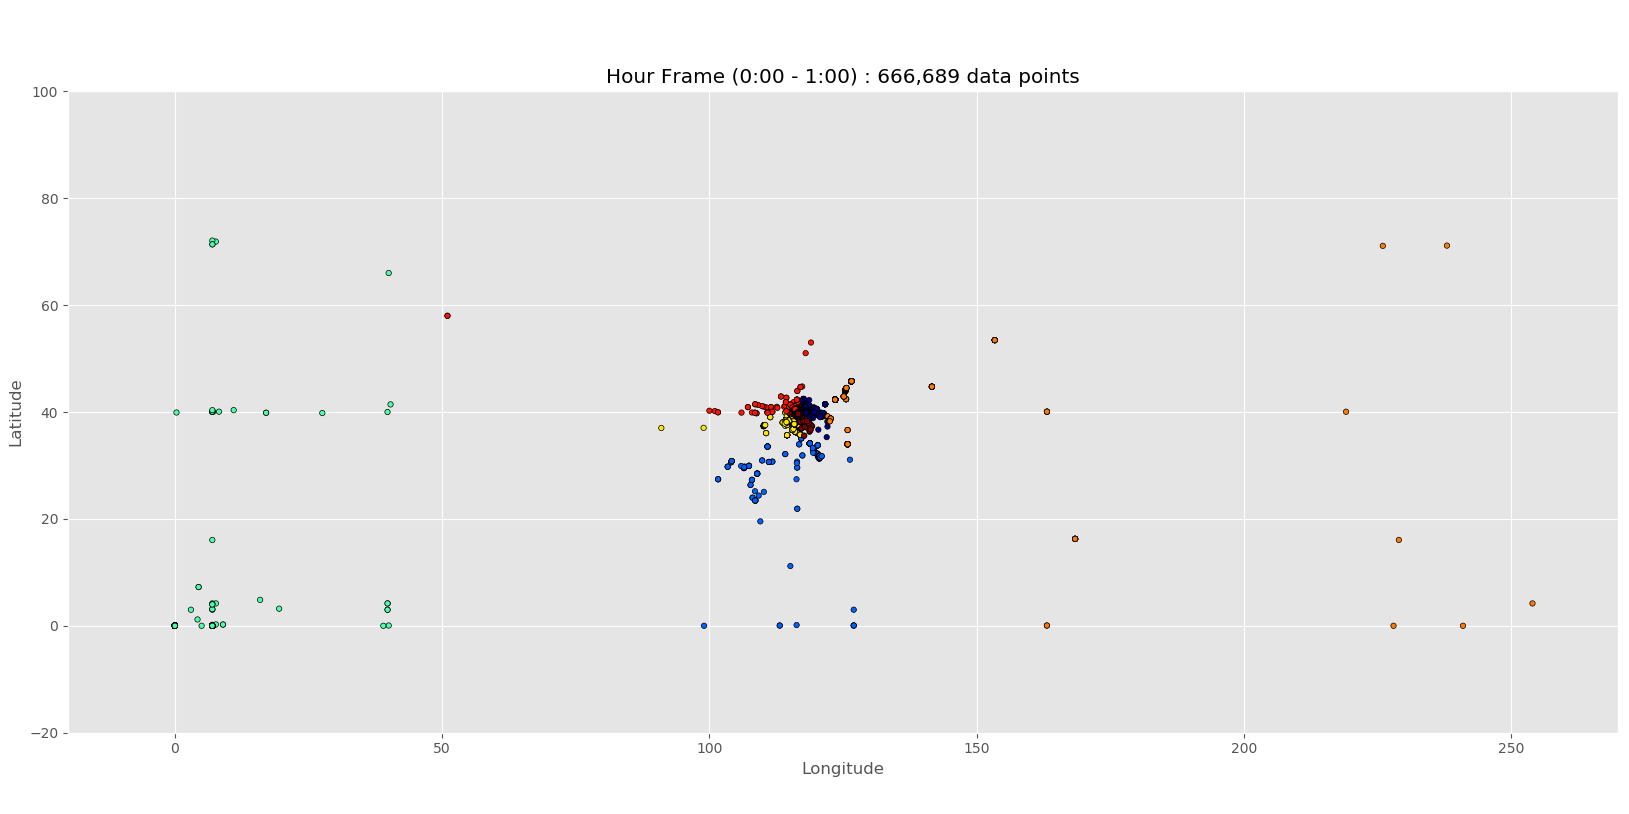
\includegraphics[width=2.5in]{image/Scatter0.png}
	\caption{The clustered GPS data points of taxi drivers in the hour frame from 0:00 to 1:00.}
	\label{fig_scatter0}
\end{figure}

\subsection{Program procedure}
The Fig.\ref{fig_workflow} illustrates insight into the working flow of our program. Firstly, we feed the .csv data file, $k$ value, and iteration value into the model. In the next stage, the class of DataFileReader.java will preprocess the raw data, which converts the data into arrays before the processing phase. The system will use the ready-to-train data in our k-means algorithm. The K-means.java class is the heart of our program, which operates and organizes sub-classes functions. 

To be more specific, the class mentioned above calls the mandatory sub-class, which is Cluster.java. This class will do the work of assigning data points and re-calculate the centroids based on the Euclidean distance method in Distance.java. Finally, when the number of iterations matches the stopping criteria, the program will print the centroid coordinates on the screen, and save the labeled data points into the format of .csv. We will introduce the detailed descriptions of our system in the following sections.

\begin{figure}[!t]
	\centering
	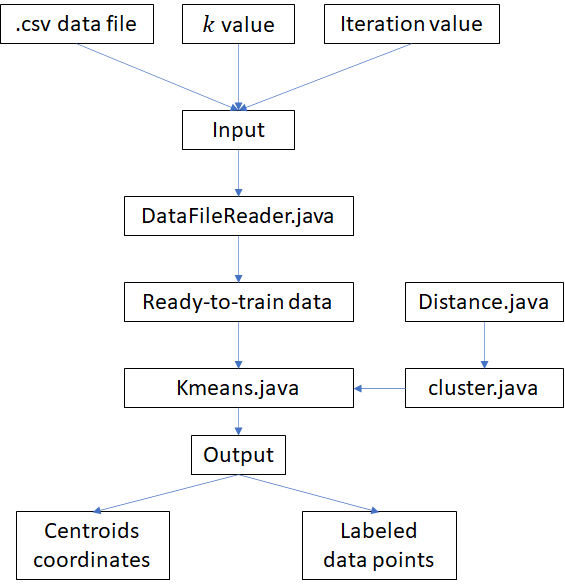
\includegraphics[width=2.5in]{image/workflow.png}
	\caption{Program work flow.}
	\label{fig_workflow}
\end{figure}

\subsubsection{DataFileReader.java}
\begin{itemize}
	\item Sub-classes: ReadCSVFile, ReadTSVFile.
	\item Main functions: 
	\subitem Convert input data file into arrays. 
	\subitem Record the number of data points and data dimension.
\end{itemize}

\subsubsection{KMeans.java}
\begin{itemize}
	\item Sub-classes: kmeans, ClusterPoints, FindNearestCentroid.
	\item Main functions:
	\subitem Performs k-means clustering on a dataset.
	\subitem Cluster all data points into their nearest centroids’ cluster.
	\subitem Calculate the nearest centroid of the candidate point, returns the cluster's index.
\end{itemize}

\subsubsection{Cluster.java}
\begin{itemize}
	\item Sub-classes: Cluster, Centroid, ArrayList, SetCentroid, Insert, SumSquareError, ClearPoints, CalcCentroid.
	\item Main functions:
	\subitem Cluster instantiation.
	\subitem Retrieve centroid (average) of the cluster as an array of coordinate values.
	\subitem Return the list of points belong to a cluster.
	\subitem Set cluster centroid with coordinates of the given centroid.
	\subitem Insert given point into the cluster.
	\subitem Returns the sum of squared errors.
	\subitem Clears points in the cluster before each iteration.
	\subitem Calculates and stores the value of the new centroid from all points.
\end{itemize}

\subsubsection{Distance.java}
\begin{itemize}
	\item Sub-classes: Euclidean
	\subitem Main Functions:
	\subitem Calculates and returns Euclidean distance between two points of equal arbitrary dimensions
	
\end{itemize}

\subsection{Program demonstration}
For a brief demonstration of the program, a procedure was introduced as below:
\begin{itemize}
	\item \textit{Step 1}: Load the project folder, clean and build the project into the .jar file.
	\begin{figure}[!t]
		\centering
		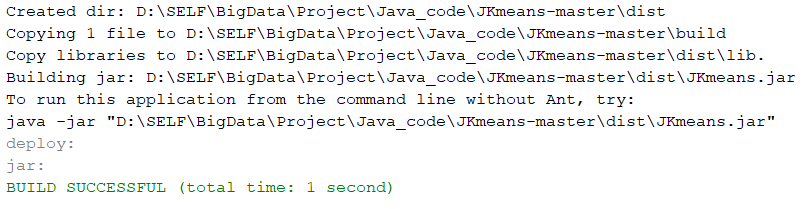
\includegraphics[width=2.5in]{image/Step1.png}
		\caption{Program demonstration step 1.}
		\label{fig_step1}
	\end{figure}

	\item \textit{Step 2}: Open the command window, run the .jar file and give the input of data path, result data path, $k$ value, and iteration value.
	\begin{figure}[!t]
		\centering
		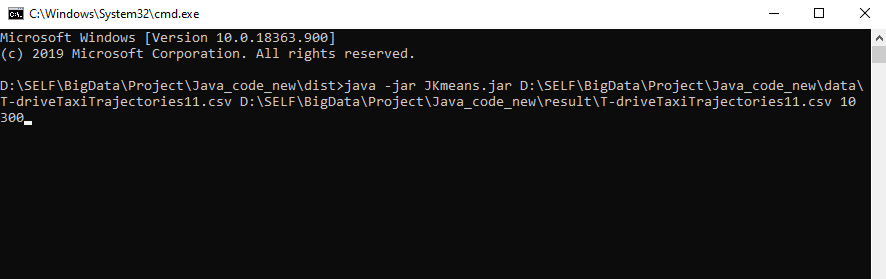
\includegraphics[width=2.5in]{image/Step2.png}
		\caption{Program demonstration step 2.}
		\label{fig_step2}
	\end{figure}
	
	\item \textit{Step 3}: the program process the $k$-means algorithm, export the centroids coordinates and labeled data points coordinates.
	\begin{figure}[!t]
		\centering
		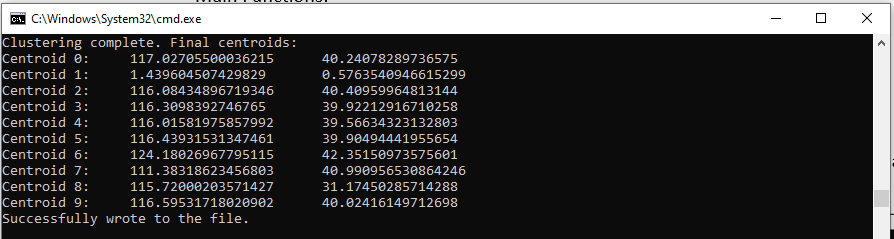
\includegraphics[width=2.5in]{image/Step3.png}
		\caption{Program demonstration step 3.}
		\label{fig_step3}
	\end{figure}
\end{itemize}

%---- Section 3 ----------------------------------------------------------------

\section{Data}
\subsection{Data}
Data in this paper was referenced from Jing Yuan et al. \cite{zheng2011t-drive} via Microsoft publication homepage. This is a sample of T-Drive trajectory dataset that contains a one-week trajectories of 10,357 taxis. The total number of points in this dataset is about 15 million and the total distance of the trajectories reaches 9 million kilometers\cite{10.1145/1869790.1869807}\cite{10.1145/2020408.2020462}.

\textit{Taxi Trajectories:} the real trajectory dataset generated by over 33,000 taxis over a period of 3 months. The total distance of the data set is more than 400 million kilometers and the total number of GPS points reaches 790 million. The average sampling interval of the data set is 3.1 minutes per point and the average distance between two consecutive points is about 600 meters. After the preprocessing, they obtain a trajectory archive containing 4.96 million trajectories. 

\textit{Real-User Trajectories:} They use a 2-month driving history of 30 real drivers recorded by GPS trajectories to evaluate travel time estimation. This data is a part of the released GeoLife data-set\cite{10.1145/1367497.1367532}\cite{10.1145/1409635.1409677}, and the average sampling interval is about 10s. That is, They can easily determine the exact road segments a driver traversed and corresponding travel times.

\subsection{Preprocessing}
The raw data includes properties: taxi id, date time, longitude, latitude. The fig.\ref{fig_rawdata} below indicates a piece of sample in a file. In this paper, we will clean the raw data and separate the data into 24 data files according to 24 time-ranges from 0:00 to 24:00. There are only 2 properties are remained: longitude and latitude.
\begin{figure}[!t]
	\centering
	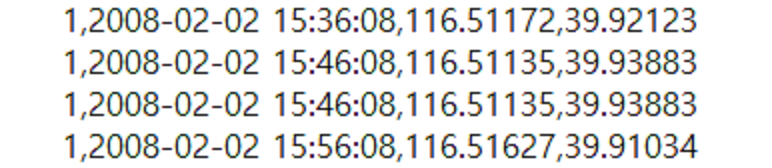
\includegraphics[width=2.5in]{image/rawdata01.png}
	\caption{Histograms of daily hour clustering .}
	\label{fig_rawdata}
\end{figure}



\section{Evaluation and results}
\subsection{Evaluation}
\label{subsection:evaluation}
Evaluating graphs: We build a set of histogram graphs with different values of time-range from 0:00 to 24:00. For intuitive visualization, we group all clustered data point into histograms as shown fig.\ref{fig_HistogramTotal} for friendly reading. After project each real-user trajectory to histogram and compare the magnitude of each cluster of each individual time-range, we find that some clusters are more significant than the others. These clusters are the one need to investigate, so, we assume that it represents its time-ranges. Using mean as a reference value of every largest cluster in each time-frame, we easily see the trend of data via the fig.\ref{fig_average}. The figure show the significantly increasing of taxi service in time-frame 13-17 respect to time-range 13:00-18:00. This specific time-range have also known as rush hours. 

\begin{figure}[!t]
	\centering
	\includegraphics[width=2.5in]{image/HistogramTotal.jpg}
	\caption{Histograms of daily hour clustering .}
	\label{fig_HistogramTotal}
\end{figure}

\begin{figure}[!t]
	\centering
	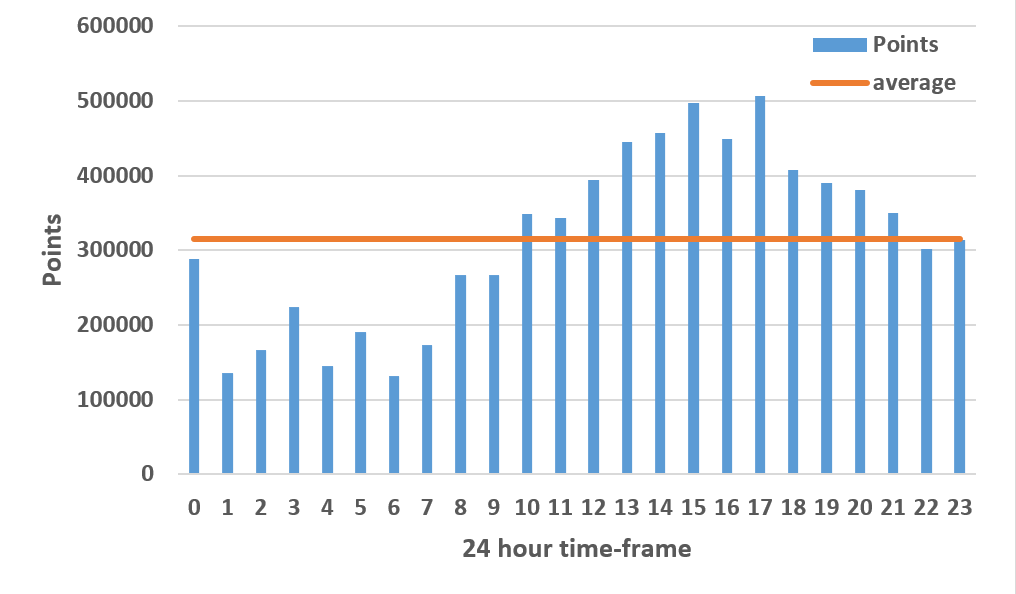
\includegraphics[width=2.5in]{image/average.png}
	\caption{All largest cluster in every time-frame and its average}
	\label{fig_average}
\end{figure}

Investigate the root cause for the high taxi demand in this time-range, we find the location ,via define on map with longitude and latitude, respect to this time range. We found that this is Xidan sub-district, a major traditional commercial area in Beijing, China. It is located in the Xicheng District. The Xidan commercial district incorporates the Xidan Culture Square, North Xidan Street, as well as many supermarkets and department stores. Understandably for the high taxi demand in this area, where people go for shopping, hanging out and have dinner. This also explain for the significantly decrease of demand after 18:00, when people are finish the activities and go home. We all know that Covid-19 start from a Wuhan's traditional market and rapidly spread out to the worlds. With high density of population, supermarkets, department stores, and restaurants, Xidan sub-district area absolutely is high risk place for Covid-19 infection. 

In addition, in different regions, the temporal characteristics of taxi demand are very different. For example, the city hall has many pick-ups, especially in the night time, namely, from 21:00 to 5:00 the next day. During this period, there is no public bus transportation, but city hall areas still gather. Oppositely, the airport area has a high pick-up ratio during the airplane arrival and departure time \cite{santani2008spatio}\cite{agarwal2004comparison}.

A gathering of all clustered GPS data points in the daily hour clustering was shown is fig.\ref{fig_ScatterResize}. This is an intuitive way to track the visual change of location distribution and see the distribution of each clustered time-frame.

\begin{figure}[!t]
	\centering
	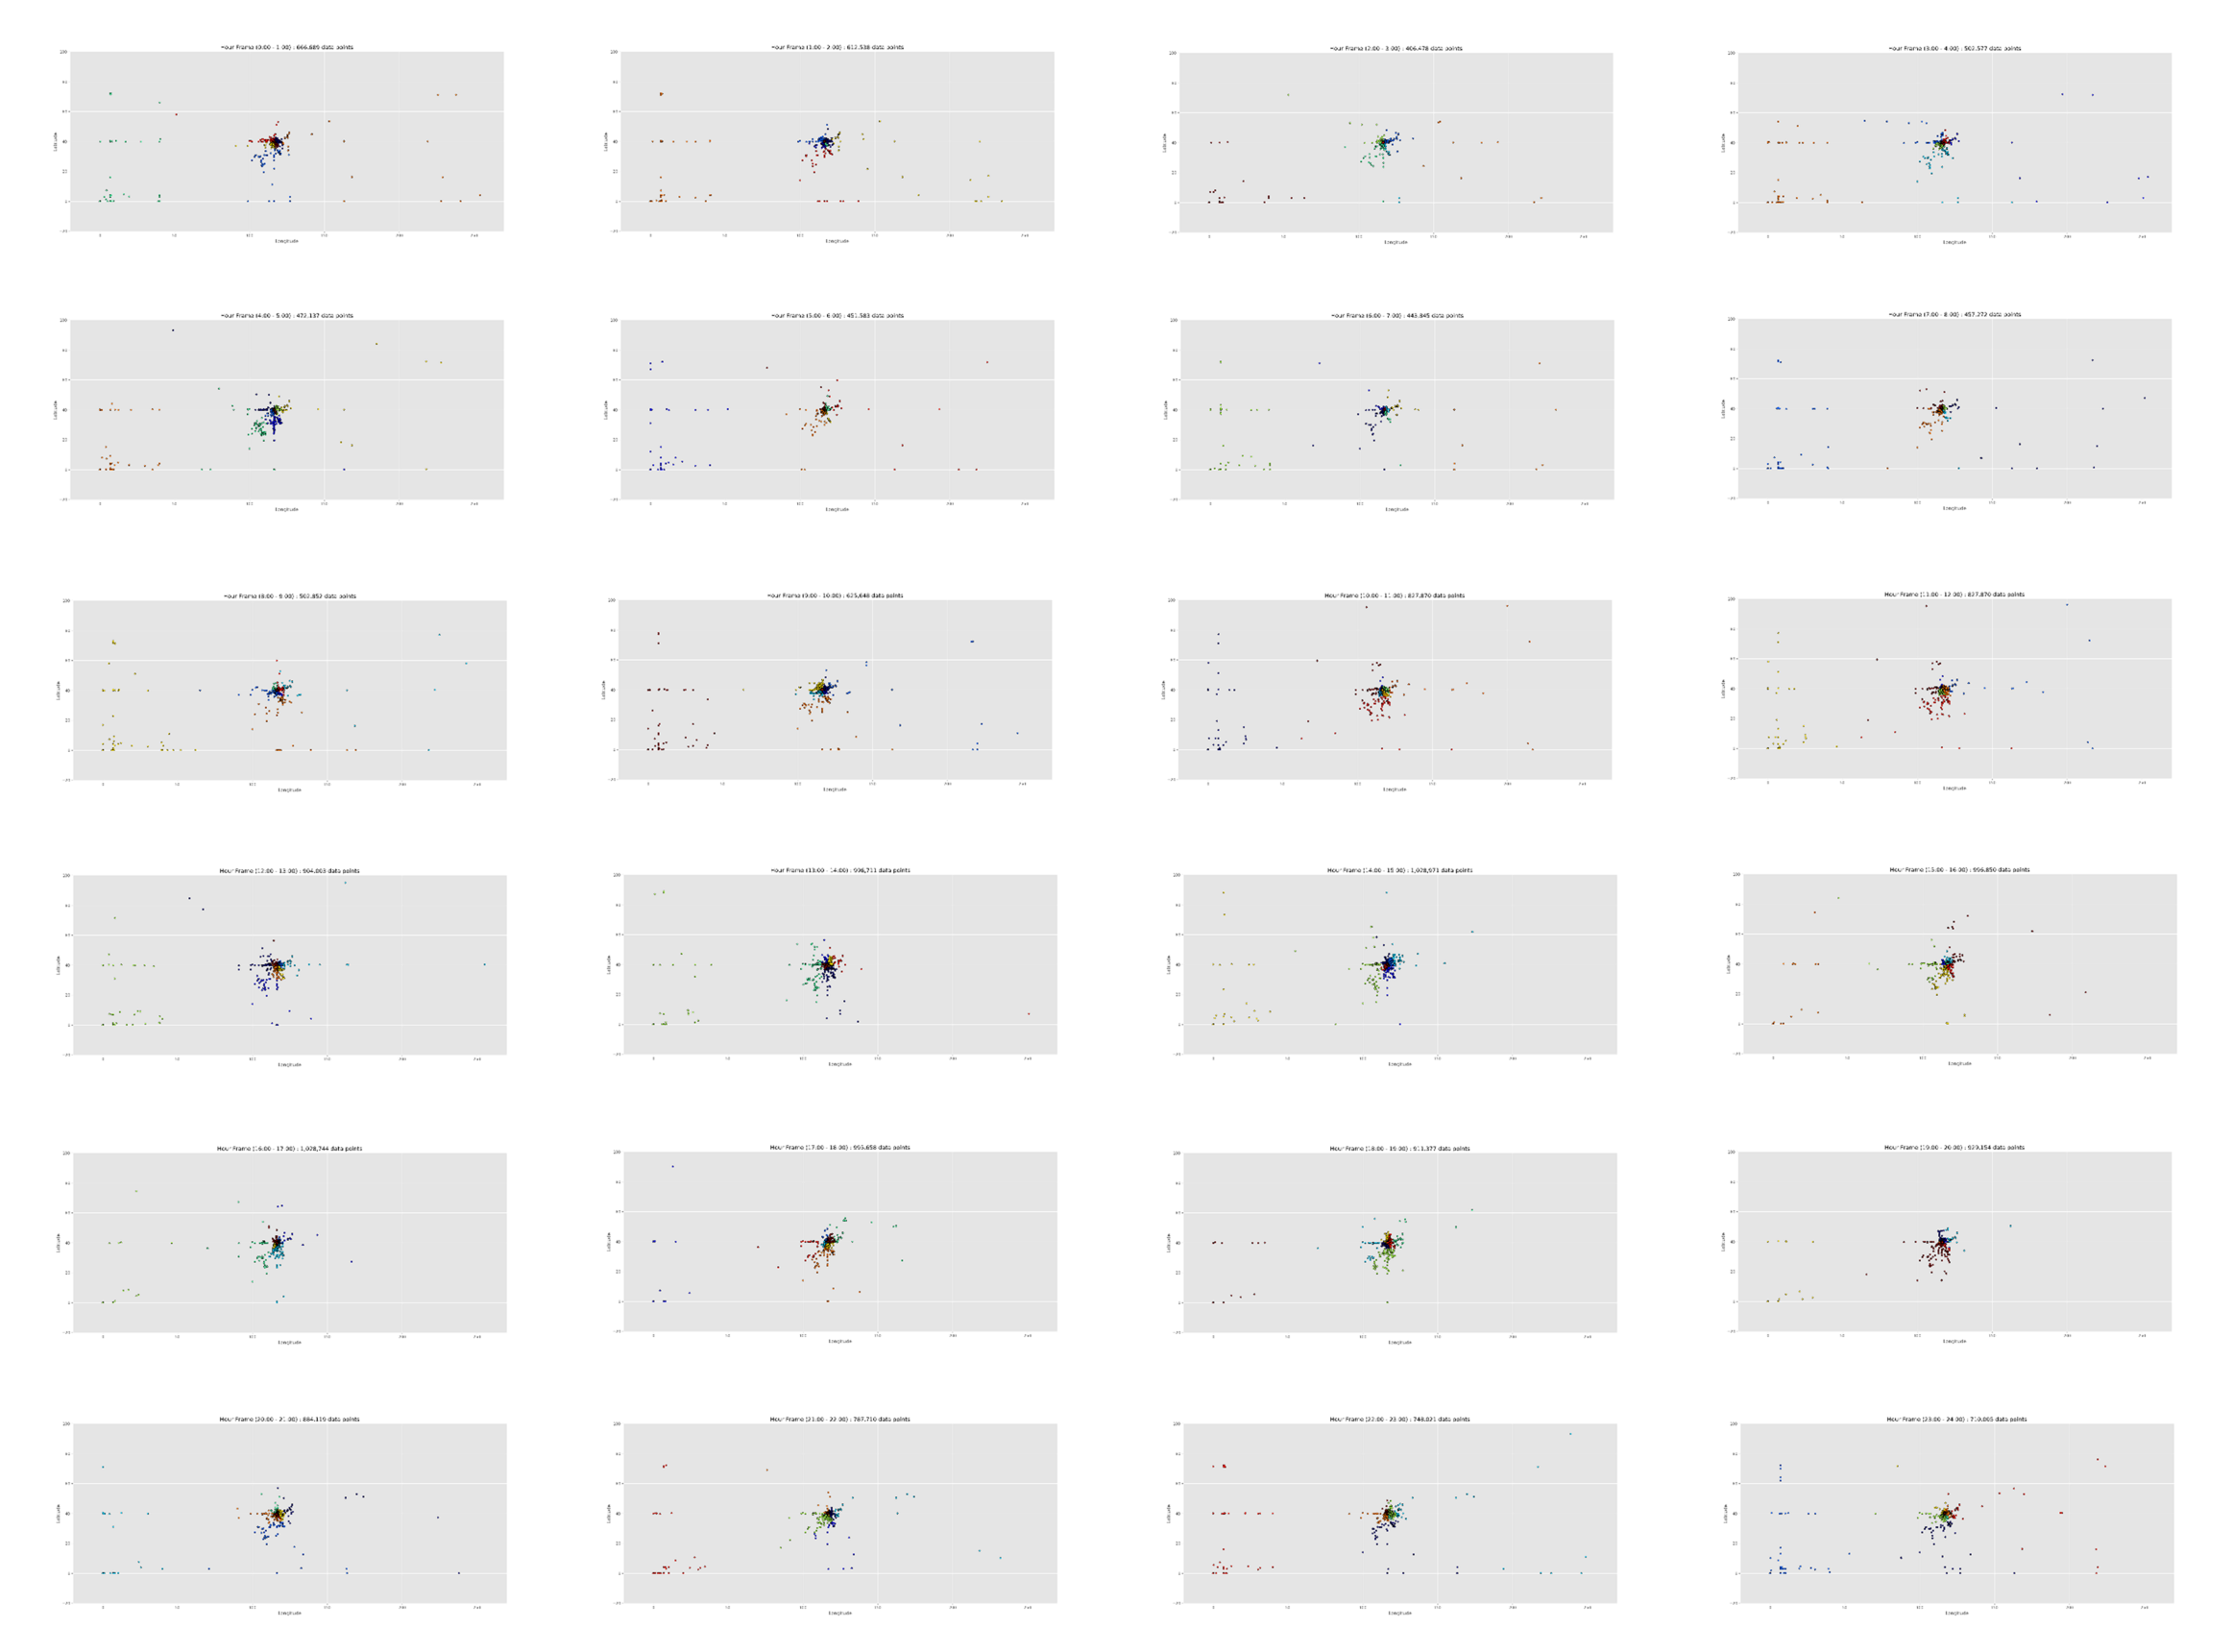
\includegraphics[width=2.5in]{image/ScatterResize.png}
	\caption{The clustered GPS data points of taxi drivers in the daily hour clustering.}
	\label{fig_ScatterResize}
\end{figure}

\subsection{Results}

Via latitude and longitude, we can find the exact location, the Sanlihe Road, 100032 Beijing, China , as shown in fig.\ref{fig_map_location13}. Vary coordinate can integrate with map to show exact location. The Sanlihe Road is part of Xicheng District, Beijing, China. The Xidan commercial district, Beijing Financial Street (Jinrongjie), Beihai Park, Jingshan Park, Shichahai and Zhongnanhai are within its jurisdiction. The popular Houhai bar area is also in Xicheng Precinct. This district is most active area in Beijing, which include 1,259,000 resident and poluation density of 25000 inhabitants per km$^2$. Others locations of each time-frame from 13 to 17 is also Xicheng District and its surrounding area with trivial distance. 

As evaluation in the subsection.\ref{subsection:evaluation} above, the peak value of the trend is time-frame 17 (which from 17:00 to 18:00). The specific histogram of clustered hour frame 17:00-18:00 was shown in the fig.\ref{fig_histogram} to point out the data distribution in each clustering. Respectively, data distribution over longitude and latitude as shown in fig.\ref{fig_scatter17}. We can visually see the dense clusters and the sparse clusters.

\begin{figure}[!t]
	\centering
	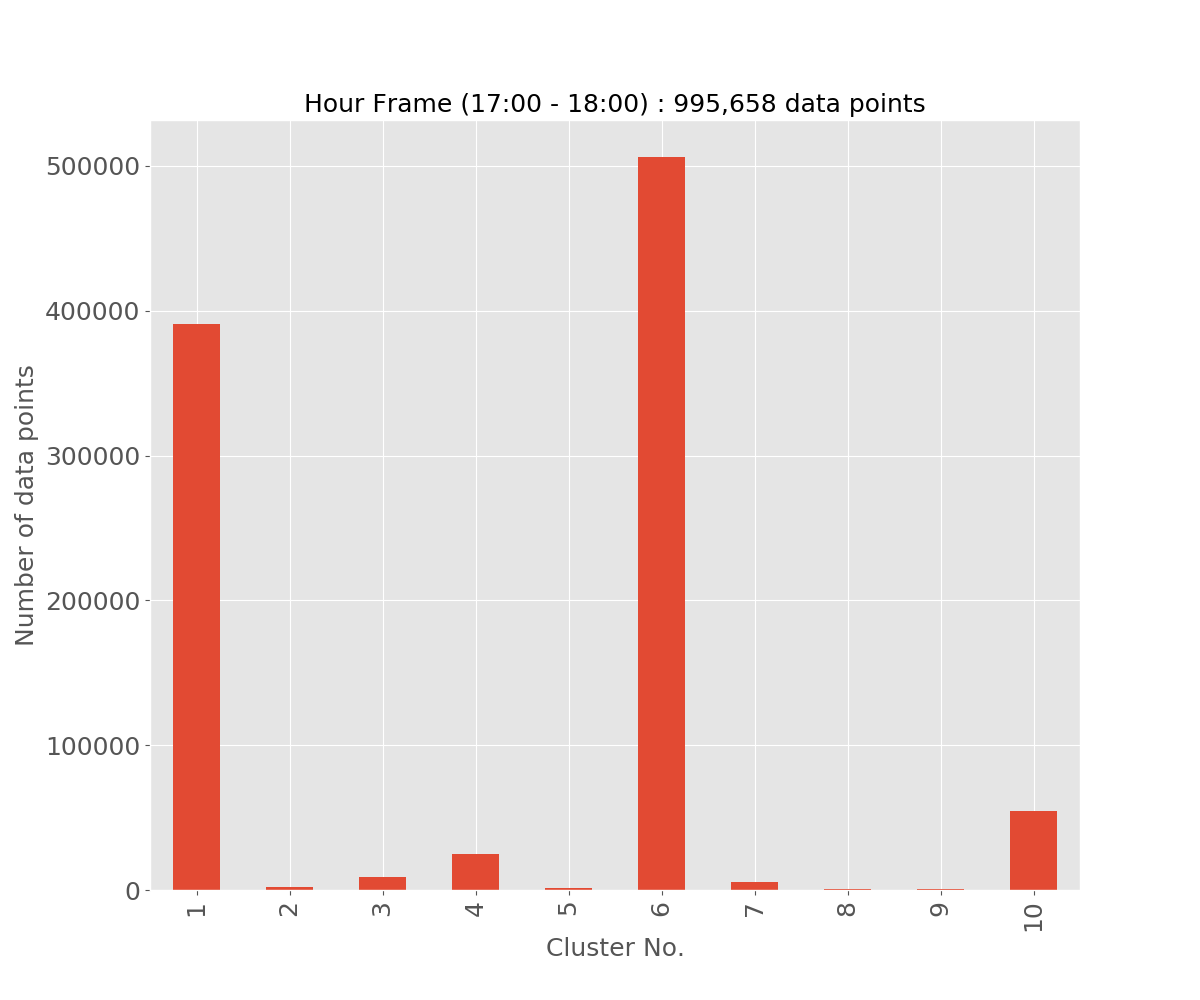
\includegraphics[width=2.5in]{image/Histogram17.png}
	\caption{Histograms for clustered hour frame 17:00-18:00.}
	\label{fig_histogram}
\end{figure}

\begin{figure}[!t]
	\centering
	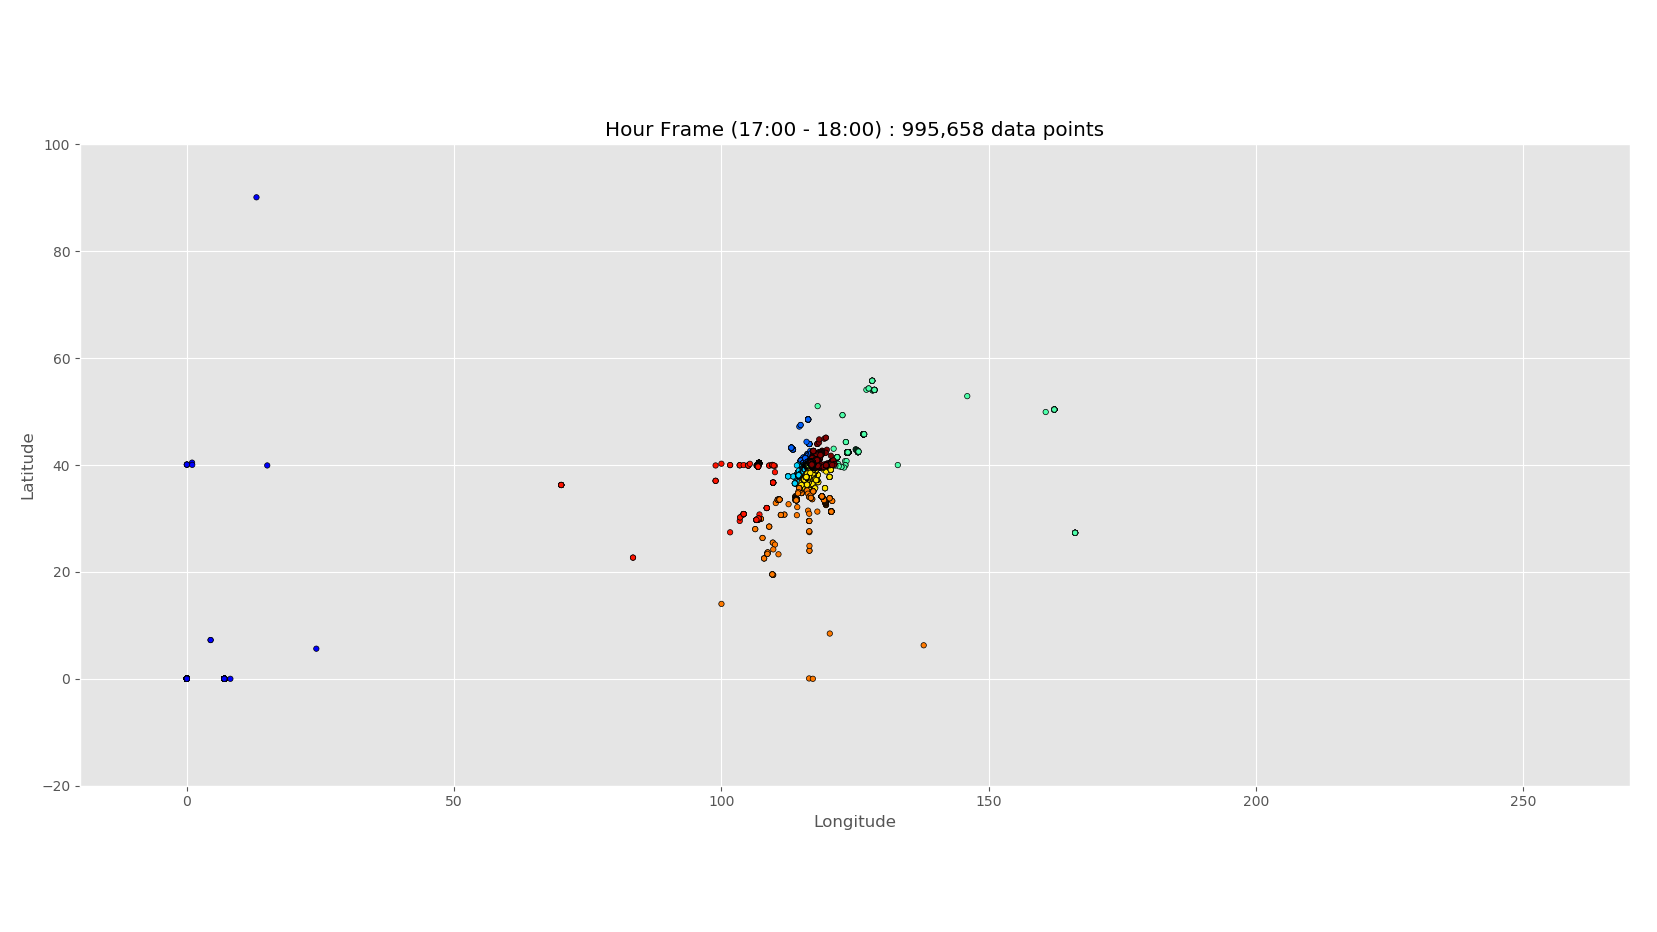
\includegraphics[width=2.5in]{image/Scatter17.png}
	\caption{The clustered GPS data points of taxi drivers in the hour frame from 17:00 to 18:00.}
	\label{fig_scatter17}
\end{figure}

Due to the research, we recommend taxi users and taxi drivers avoid to enter this area from 13:00 to 18:00 or they may come in another time. If there are unavoidable affair in this area, wearing marks, bringing hand sanitizer as precautions are suggested.

\begin{figure}[!t]
	\centering
	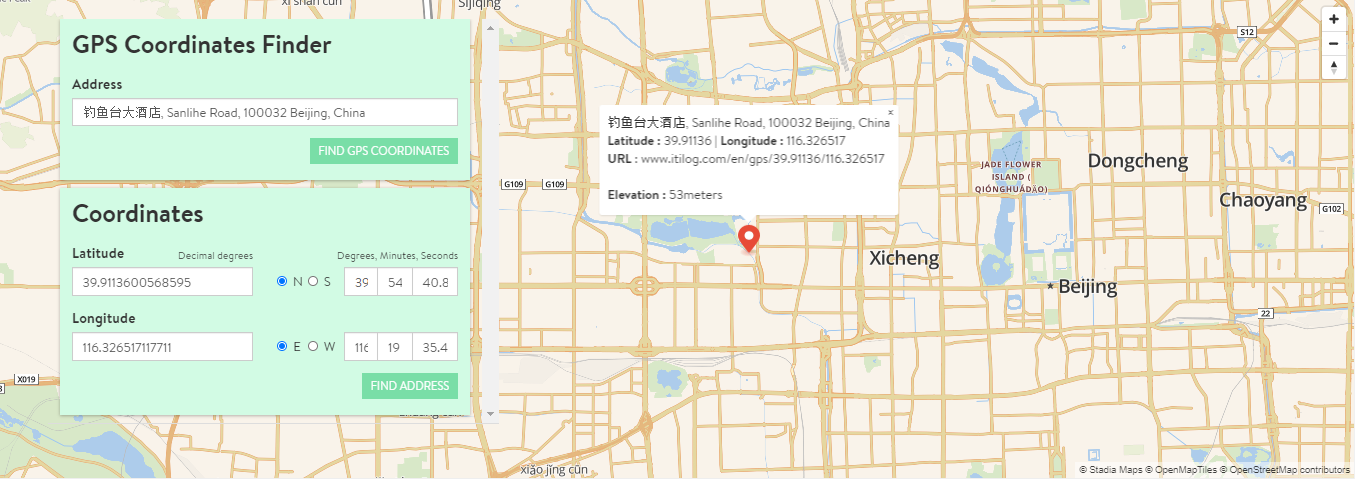
\includegraphics[width=2.5in]{image/map_13.png}
	\caption{Define location on map with latitude and longitude of time-frame 13.}
	\label{fig_map_location13}
\end{figure}



%\begin{figure}[!t]
%	\centering
%	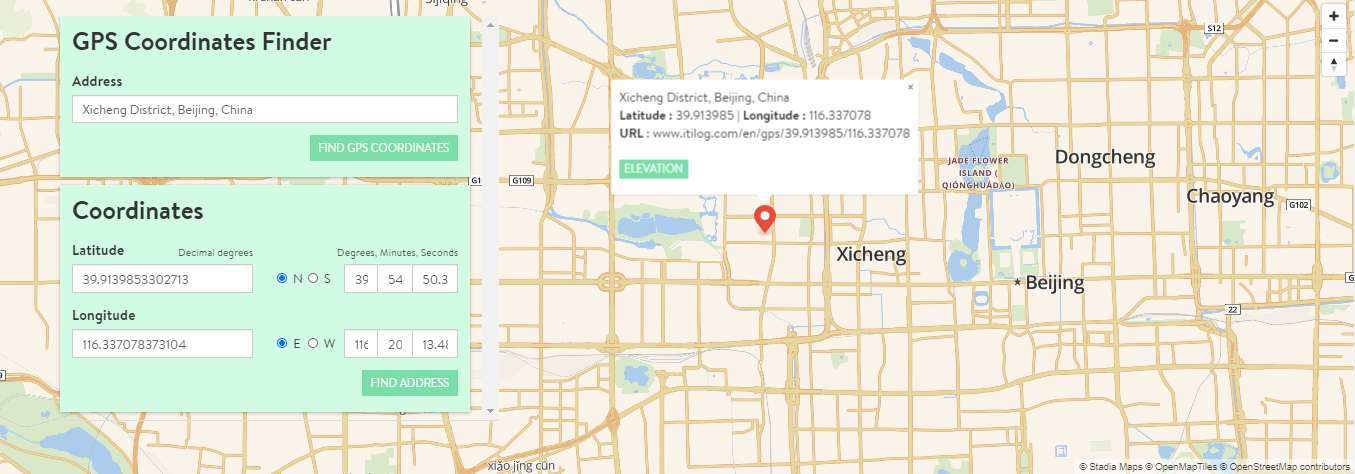
\includegraphics[width=2.5in]{image/map_17.png}
%	\caption{Define location on map with latitude and longitude of time-frame 17.}
%	\label{fig_map_location17}
%\end{figure}

%---- Section 5 ----------------------------------------------------------------

\section{Conclusion}


This paper presents an approach that finds out the practically crowded area at a specific time-range in terms of taxi drivers’ intelligence learned from a large number of historical taxi trajectories. We first group data points with clustering method to crowded area. We evaluate the results to find the specific time-range. The results show that our method can give a brief recommendation in the aspects of effectiveness and efficiency. We agree that a recommended crowded area would become less dangerous if many people avoid it. The given recommendation is taxi users and taxi drivers avoid to enter this area from 13:00 to 18:00 or they may come in another time. This is recommendation may change taxi user decision and lead to the changing of taxi driver operation. The system will adapt and give the updated recommendation. In the future, integrate map to find moving route, moving frequency, and combining real-time traffic information with our approach to help taxi driver avoid potential infection area. 


% if have a single appendix:
%\appendix[Proof of the Zonklar Equations]
% or
%\appendix  % for no appendix heading
% do not use \section anymore after \appendix, only \section*
% is possibly needed

% use appendices with more than one appendix
% then use \section to start each appendix
% you must declare a \section before using any
% \subsection or using \label (\appendices by itself
% starts a section numbered zero.)
%
%---- \appendices --------------------------------------------------------------

\appendices
\section{for Java code and data sample}
Code and data can be found and downloaded via github: \url{https://github.com/dophuan/t-drive}.


%\begin{lstlisting}[language=Python]
%package jkmeans;
%
%import java.io.File;
%import java.io.FileWriter;
%import java.util.Random;
%import java.io.IOException;
%import java.util.ArrayList;
%
%/**
%* This class demonstrates the use of the Kmeans library and helper classes. Based on code written Fall 2012.
%*/
%
%public class Tester {
%
%private static int[] seeds;
%
%public static void main(String[] args) {
%//Grab params here, add bounds checking
%String filename = args[0];
%String dir = args[1];
%int k = Integer.parseInt(args[2]);
%int i = Integer.parseInt(args[3]);
%
%//Use DataFileReader to process data file into double[][].
%double[][] data = DataFileReader.ReadCSVFile(new File(filename));
%int n = data.length;
%
%//Choose initial seeds for cluster centroids.
%randomSeeds(k, n);  //This will eventually be replaced by k-means++
%
%//Grab a list of the final centroids after clustering.
%Cluster[]clusters = KMeans.kmeans(data, k, i, seeds);
%double[][]centroids = new double[clusters.length][2]; //Clustering executed in this line
%
%for (int m = 0; m < k; m++) {
%centroids[m] = clusters[m].Centroid();
%}
%
%//Print output
%System.out.println("Clustering complete. Final centroids:");
%
%for (int j = 0; j < centroids.length; j++) {
%StringBuilder line = new StringBuilder();
%line.append("Centroid ");
%line.append(j);
%line.append(": ");
%
%for (int m = 0; m < centroids[0].length; m++) {
%line.append("\t");
%line.append(centroids[j][m]);
%}
%
%System.out.println(line.toString());
%}
%
%
%try {
%File myFile = new File(dir);
%myFile.createNewFile();
%
%FileWriter myWrite = new FileWriter(dir);
%for (int j = 0; j < clusters.length; j++) {
%ArrayList<double[]> points = clusters[j].GetPoints();
%for (int iter = 0; iter < points.size(); iter++) {
%double[] point = points.get(iter);
%myWrite.write(point[0] + ", " + point[1] + ", " + (j+1) + "\n");
%}
%
%}
%myWrite.close();
%System.out.println("Successfully wrote to the file.");
%} catch (IOException e) {
%System.out.println("An error has occurred");
%e.printStackTrace();
%}
%}
%
%/**
%* This method randomly selects the indices of K points to use as the initial centroids for seeding.
%* @param k Number of clusters that exist in the data.
%* @param n Total number of candidate points in the data.
%*/
%private static void randomSeeds(int k, int n) {
%seeds = new int[k];
%int count = 0;
%
%//Randomly choose k points to be centroids. After each choice, check to see if index
%//has already been used. If so, choose another.
%while (count < k) {
%boolean uniqueIndex = true;
%Random rand = new Random();
%int index = rand.nextInt(n);
%
%//Check for uniqueness
%for (int i = 0; i < count; i++) {
%if (index == seeds[i]) {
%uniqueIndex = false;
%}
%}
%
%//If unique, add index and continue
%if(uniqueIndex) {
%seeds[count] = index;
%count++;
%}
%}
%}
%}
%\end{lstlisting}


% you can choose not to have a title for an appendix
% if you want by leaving the argument blank
%\section{}
%Appendix two text goes here.


% use section* for acknowledgment
\section*{Acknowledgment}

The authors would like to thank Prof. Joonho Kwon with the School of Computer Science and Engineering, Pusan National University, Pusan, Korea for the Big data course. The authors also thank everyone in the team for the endless efforts to finish this final project.

% Can use something like this to put references on a page
% by themselves when using endfloat and the captionsoff option.
\ifCLASSOPTIONcaptionsoff
  \newpage
\fi



% trigger a \newpage just before the given reference
% number - used to balance the columns on the last page
% adjust value as needed - may need to be readjusted if
% the document is modified later
%\IEEEtriggeratref{8}
% The "triggered" command can be changed if desired:
%\IEEEtriggercmd{\enlargethispage{-5in}}

% references section

% can use a bibliography generated by BibTeX as a .bbl file
% BibTeX documentation can be easily obtained at:
% http://mirror.ctan.org/biblio/bibtex/contrib/doc/
% The IEEEtran BibTeX style support page is at:
% http://www.michaelshell.org/tex/ieeetran/bibtex/
%\bibliographystyle{IEEEtran}
% argument is your BibTeX string definitions and bibliography database(s)
%\bibliography{IEEEabrv,../bib/paper}
%
% <OR> manually copy in the resultant .bbl file
% set second argument of \begin to the number of references
% (used to reserve space for the reference number labels box)



%----------------------------------------------------------------------------------------
%	BIBLIOGRAPHY
%----------------------------------------------------------------------------------------

%\begin{thebibliography}{1}
%\bibitem{IEEEhowto:kopka}
%H.~Kopka and P.~W. Daly, \emph{A Guide to \LaTeX}, 3rd~ed.\hskip 1em plus
%0.5em minus 0.4em\relax Harlow, England: Addison-Wesley, 1999.
%\end{thebibliography}


\bibliographystyle{IEEEtran}
%\bibitem{IEEEhowto:kopka}
\bibliography{bib}

%----------------------------------------------------------------------------------------





% biography section
% 
% If you have an EPS/PDF photo (graphicx package needed) extra braces are
% needed around the contents of the optional argument to biography to prevent
% the LaTeX parser from getting confused when it sees the complicated
% \includegraphics command within an optional argument. (You could create
% your own custom macro containing the \includegraphics command to make things
% simpler here.)
%\begin{IEEEbiography}[{\includegraphics[width=1in,height=1.25in,clip,keepaspectratio]{mshell}}]{Michael Shell}
% or if you just want to reserve a space for a photo:

\begin{IEEEbiography}[{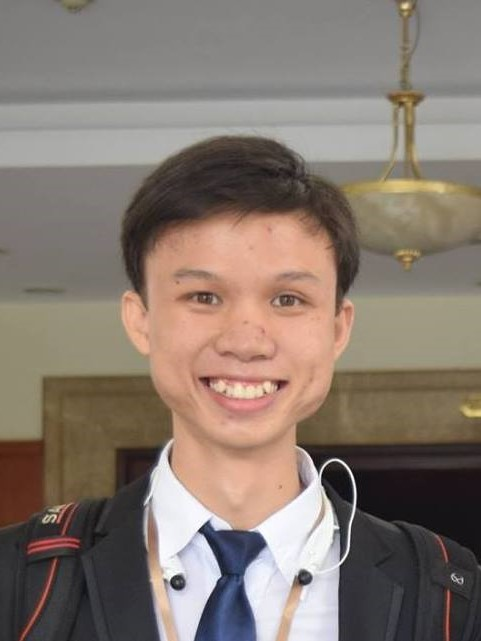
\includegraphics[width=1in,height=1.25in,clip,keepaspectratio]{image/DoPhuAn3x4}}]{Do Phu An}
is a Ph.D. candidate in Computer Engineering at the Pusan National University. He completed undergraduate study at University of Information Technology VNU-HCM. He works on the big data analysis, AI, and digital image processing. 
\end{IEEEbiography}

\begin{IEEEbiography}[{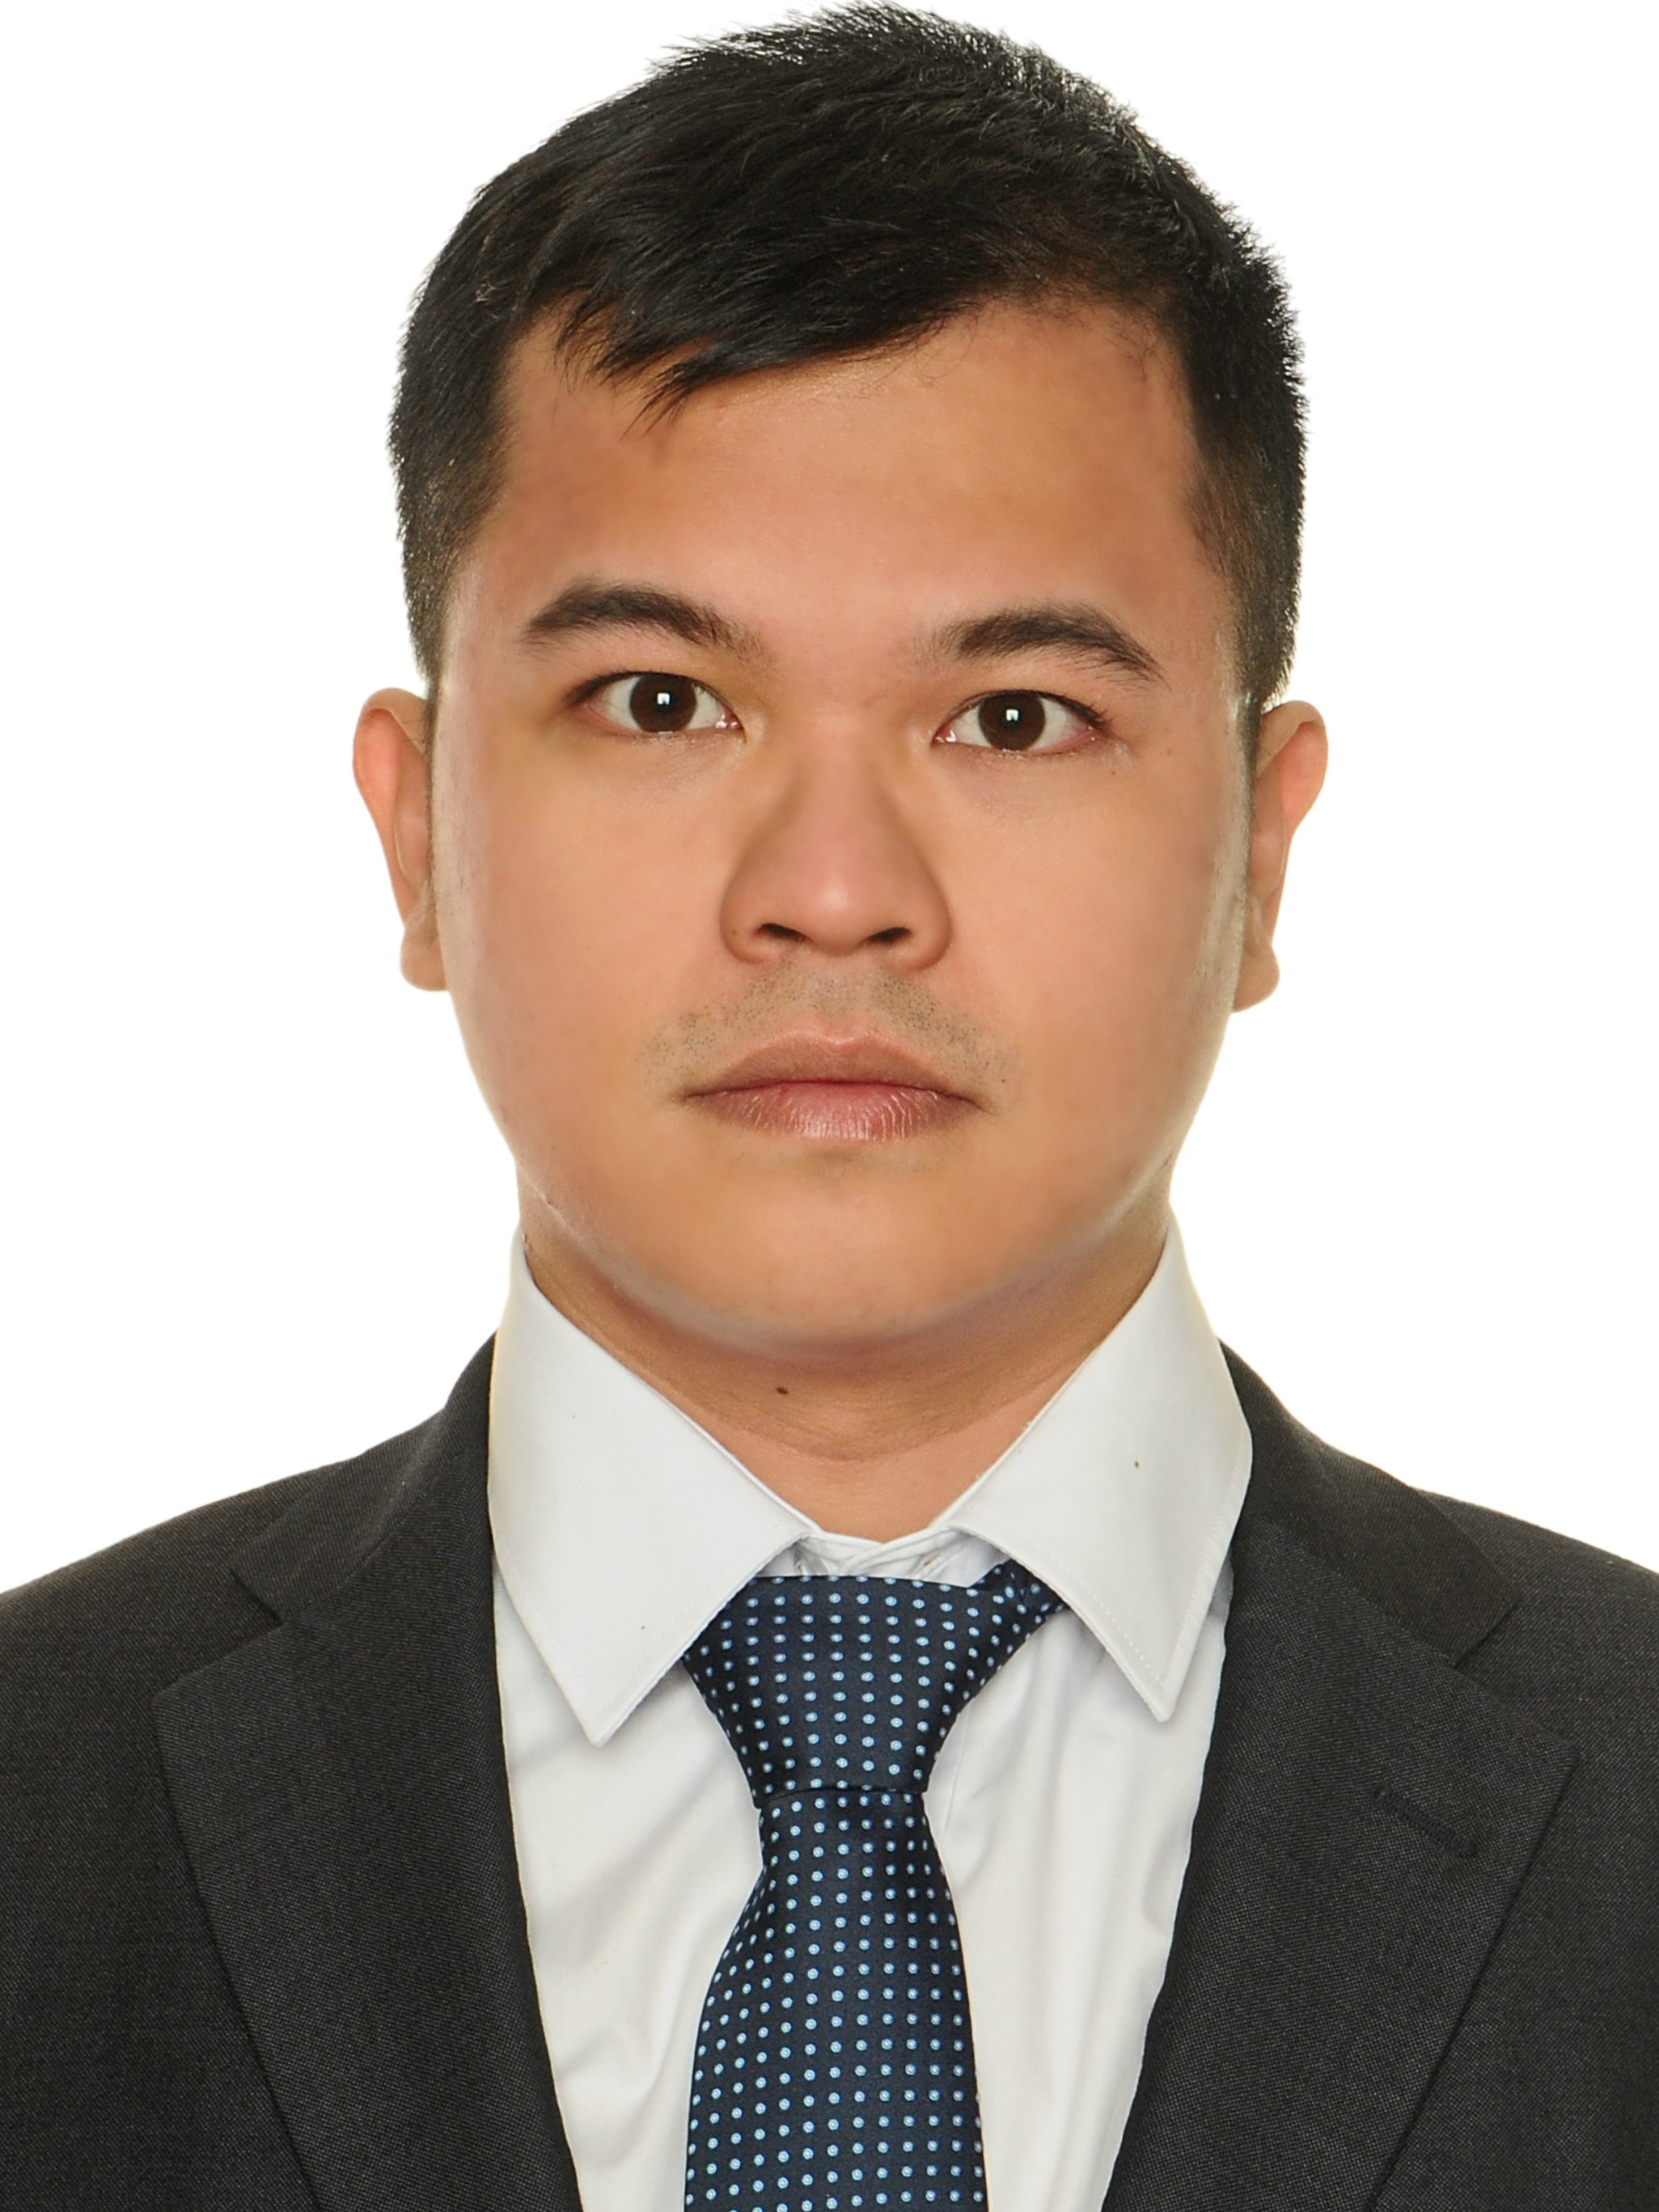
\includegraphics[width=1in,height=1.25in,clip,keepaspectratio]{image/PhamXuanQuang3x4.png}}]{Pham Xuan Quang}
is a Ph.D. candidate in Aerospace Engineering at the Pusan National University. He completed undergraduate study at Ho Chi Minh City University of Technology and his Master of Engineering at Institut Teknologi Bandung. He works on the finite element method, composite behavior, and reduced basis method. 
\end{IEEEbiography}

\begin{IEEEbiography}[{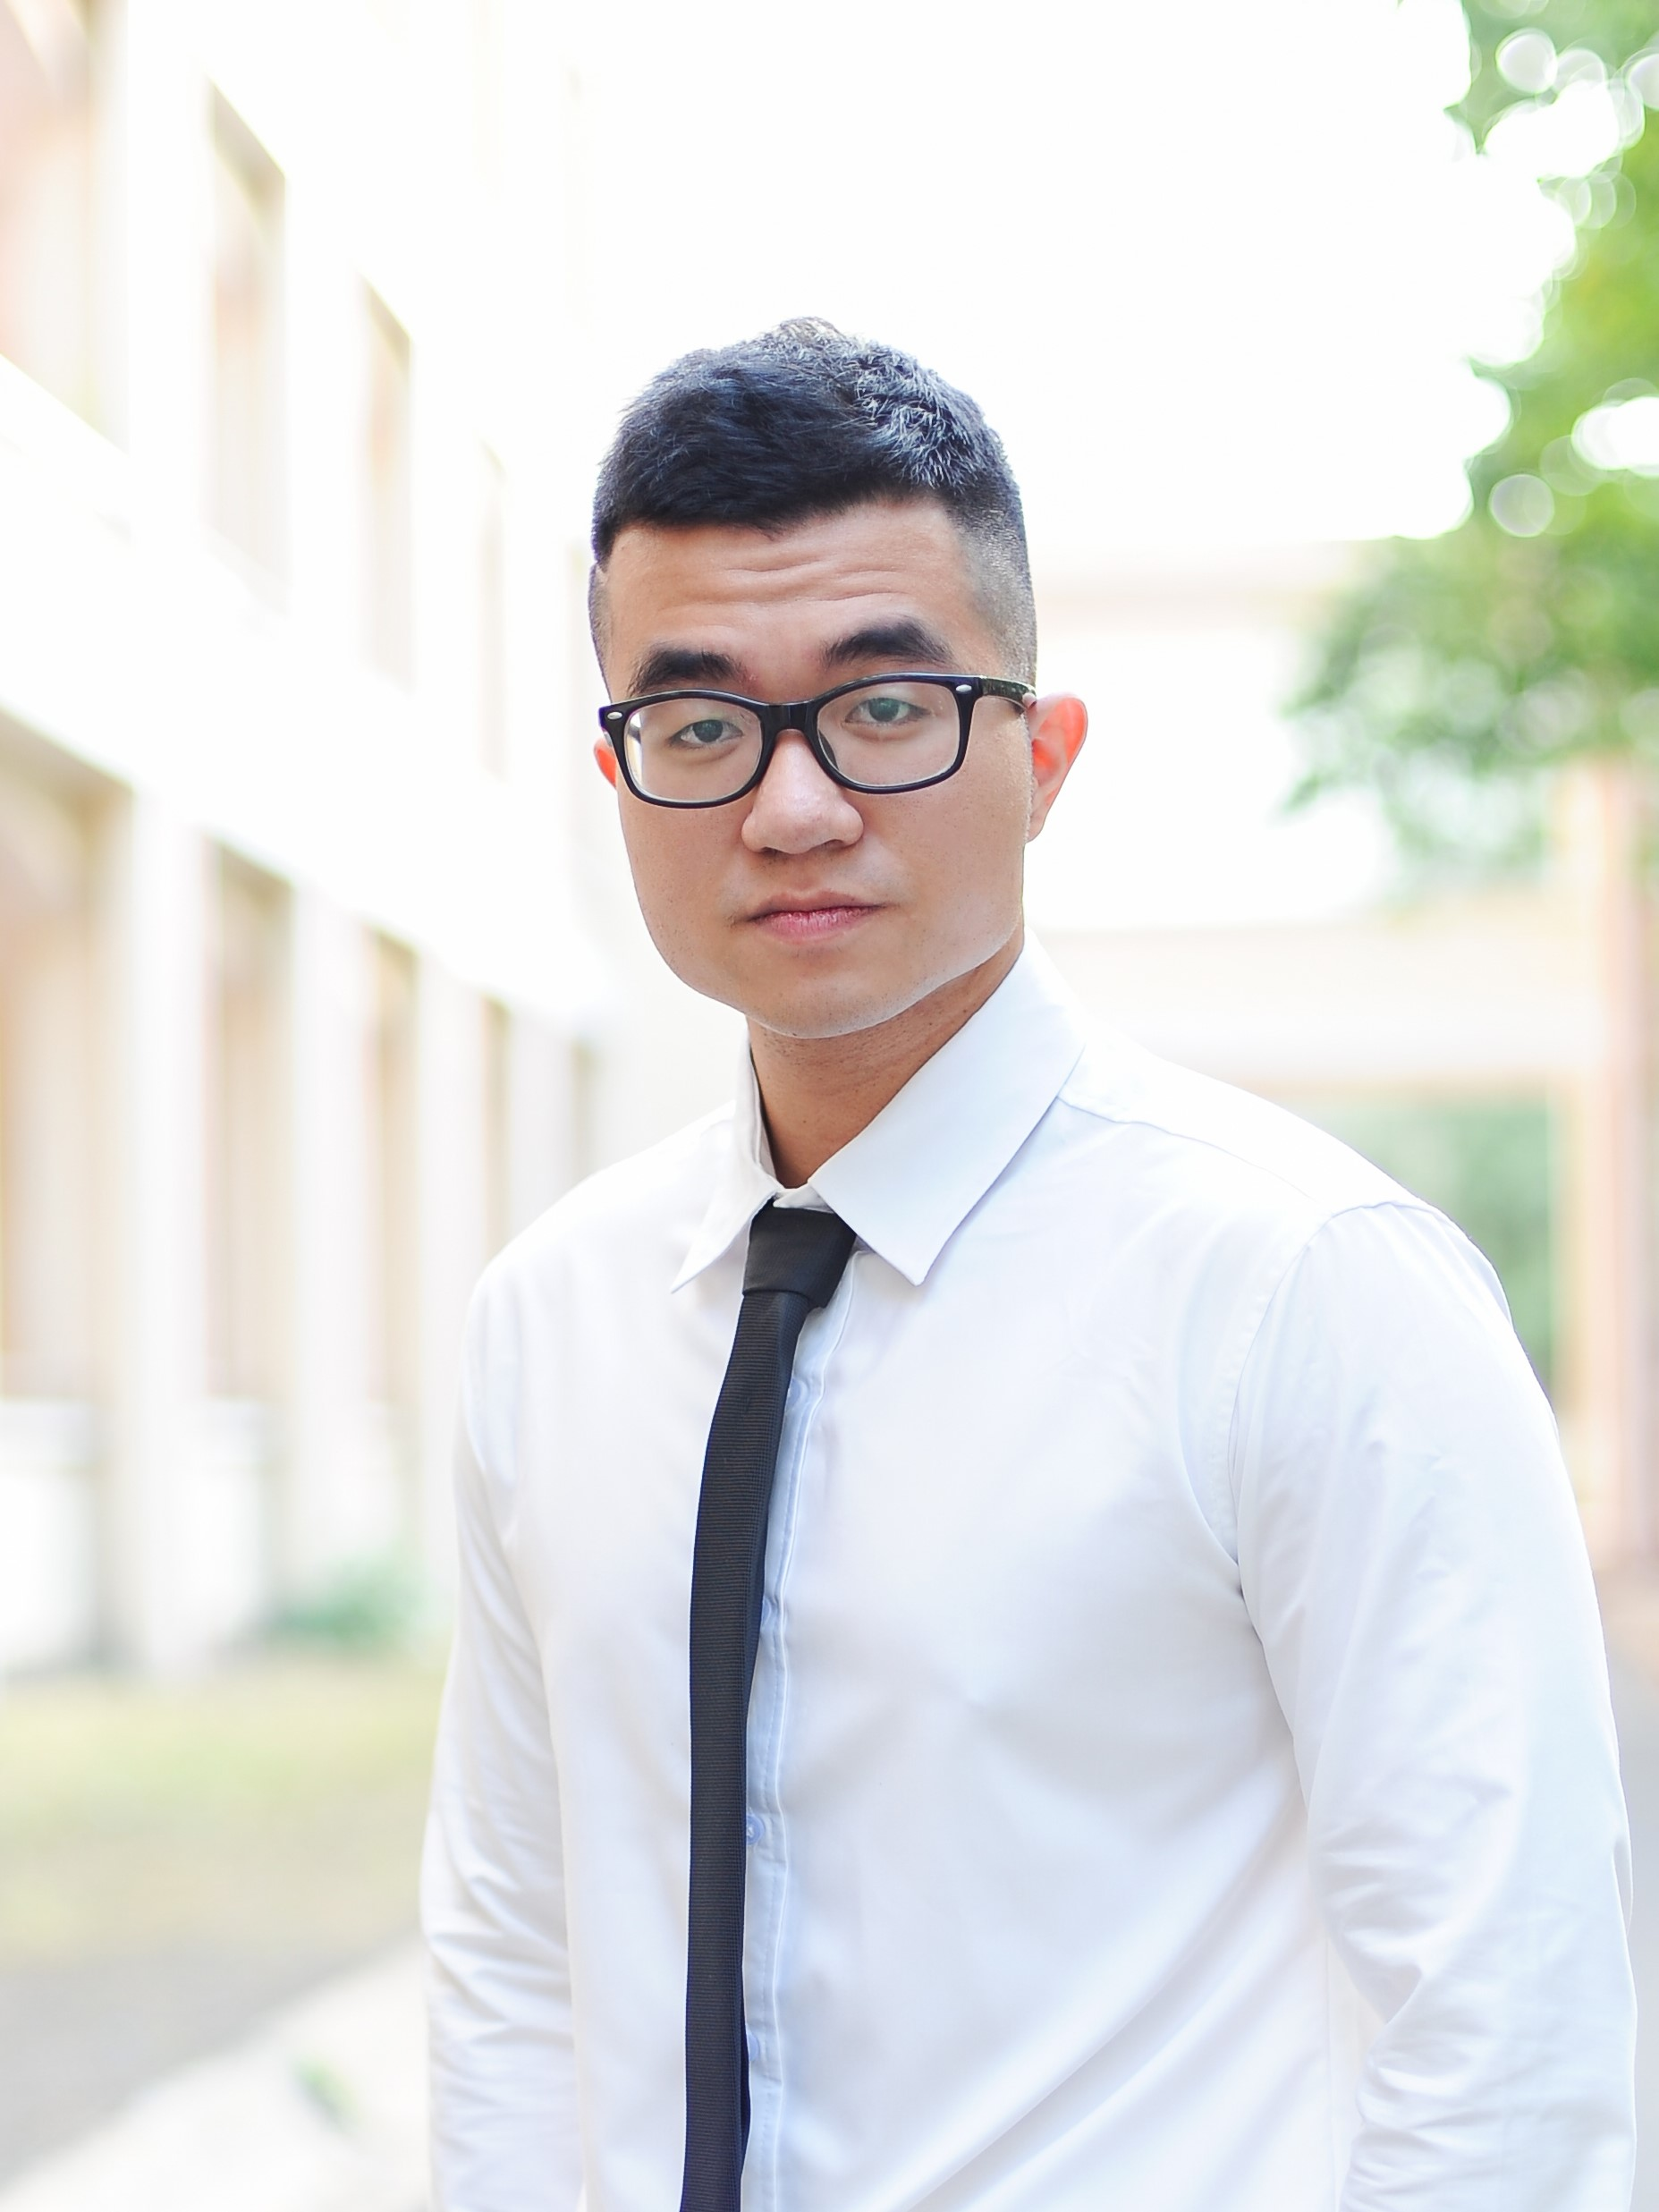
\includegraphics[width=1in,height=1.25in,clip,keepaspectratio]{image/LEHAISON3x4.png}}]{Le Hai Son}
is a Master student in Aerospace Engineering at the Pusan National University. He completed his undergraduate program at Ho Chi Minh City University of Technology. His research focuses on machine learning, deep learning applications in computer vision.
\end{IEEEbiography}

% if you will not have a photo at all:
%\begin{IEEEbiographynophoto}{Do Phu An}
%	Biography text here.
%\end{IEEEbiographynophoto}

%\begin{IEEEbiographynophoto}{Pham Xuan Quang}
%Pham Xuan Quang is a Ph.D. candidate in Aerospace at the Pusan National University. He completed undergraduate study at Ho Chi Minh City University of Technology and his Master of Engineering at Institut Teknologi Bandung. He works on the finite element method, composite behavior, and reduced basis method. 
%\end{IEEEbiographynophoto}

% insert where needed to balance the two columns on the last page with
% biographies
%\newpage

%\begin{IEEEbiographynophoto}{Le Hai Son}
%Biography text here.
%\end{IEEEbiographynophoto}

% You can push biographies down or up by placing
% a \vfill before or after them. The appropriate
% use of \vfill depends on what kind of text is
% on the last page and whether or not the columns
% are being equalized.

%\vfill

% Can be used to pull up biographies so that the bottom of the last one
% is flush with the other column.
%\enlargethispage{-5in}



% that's all folks
\end{document}









